\documentclass[a4paper,10pt]{extarticle}
\usepackage[utf8]{inputenc}
\usepackage[brazilian]{babel}

\title{IF675 - Sistemas Digitais}
\author{Luan Alves Rodrigues }
\date{Novembro de 2019}

\usepackage{natbib}
\usepackage{graphicx}
\usepackage{url}

\begin{document}

\maketitle

\section{Introdução}
A cadeira de Sistemas Digitais do curso de Ciência da Computação do Cin , ministrada pelo professor Manoel Eusébio, abrange o conhecimento de circuitos lógicos digitais combinacionais e sequenciais \citep{sistemas}. Nessa disciplina os alunos irão aprender sobre como funcionam os sistemas embarcados através de aulas teóricas e práticas\citep{SiteDisciplina}, além do trabalho em grupo. Uma das referências dessa cadeira é o livro "Introdução aos Sistemas Digitais" \citep{Livro}.

\begin{figure}[h!]
\centering
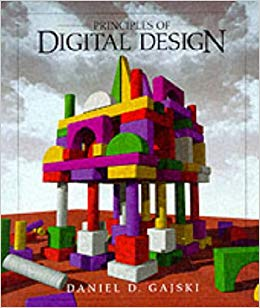
\includegraphics[scale=0.7]{1}
\caption{Principles of Digital Design\citep{Imagem}}
\label{fig:1}
\end{figure}


\section{Relevância}
Essa disciplina é importante pois ela fornece aos alunos conhecimento teórico e prático sobre sistemas embarcados, além mostrar as diferença entre os sistemas digitais e os sistemas analógicos, e apresentar o porquê da informação digital ser bem mais eficiente que a analógica.

\section{Relação com outras disciplinas}
\begin{table}[h]
 \centering
 {\renewcommand\arraystretch{1.25}
 \begin{tabular}{ l l }
  \cline{1-1}\cline{2-2}  
    \multicolumn{1}{|p{3.850cm}|}{Disciplina \centering } &
    \multicolumn{1}{p{4.217cm}|}{Relação \centering }
  \\  
  \cline{1-1}\cline{2-2}  
    \multicolumn{1}{|p{3.850cm}|}{IF674 - Infra-Estrutura de Hardware} &
    \multicolumn{1}{p{4.217cm}|}{Nessa cadeira os alunos irão usar a base de Sistemas Digitais pra se aprofundar no estudo de Hardware}
  \\  
  \cline{1-1}\cline{2-2}  
    \multicolumn{1}{|p{3.850cm}|}{IF729 -Prototip. de Circuitos Integrados} &
    \multicolumn{1}{p{4.217cm}|}{Nessa cadeira os alunos irão se aprofundar mais no conhecimentos de Sistemas Embarcados}
  \\ 
  \hline

 \end{tabular} }
\end{table}


\bibliographystyle{plain}
\bibliography{lar2}
\end{document}
